\documentclass{beamer}

\usepackage{graphicx}
\usepackage{caption}

\begin{document}
	
	\begin{frame}[plain]
		\begin{figure}
			\centering
			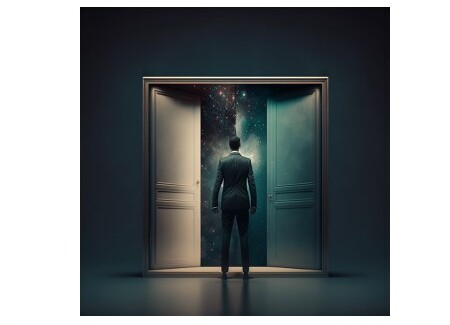
\includegraphics[width=\textwidth,height=0.85\textheight,keepaspectratio]{31.jpg}
			\caption{A man standing in front of an infinite 2D wardrobe}
		\end{figure}
	\end{frame}
	
	\begin{frame}[plain]
		\begin{figure}
			\centering
			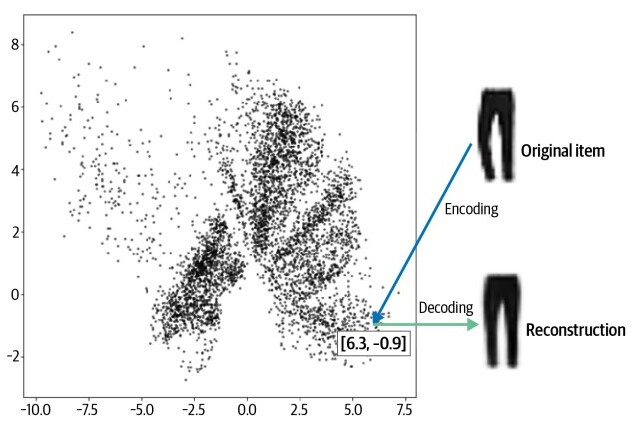
\includegraphics[width=\textwidth,height=0.85\textheight,keepaspectratio]{32.jpg}
			\caption{Items of clothing in the infinite wardrobe—each black dot represents an item
				of clothing}
		\end{figure}
	\end{frame}
	
	\begin{frame}[plain]
		\begin{figure}
			\centering
			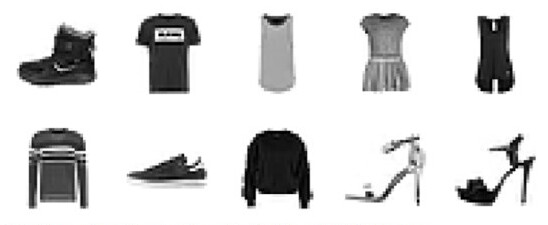
\includegraphics[width=\textwidth,height=0.85\textheight,keepaspectratio]{33.jpg}
			\caption{Examples of images from the Fashion-MNIST dataset}
		\end{figure}
	\end{frame}
	
	\begin{frame}[plain]
		\begin{figure}
			\centering
			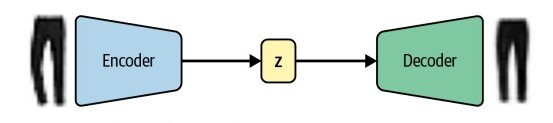
\includegraphics[width=\textwidth,height=0.85\textheight,keepaspectratio]{34.jpg}
			\caption{Autoencoder architecture diagram}
		\end{figure}
	\end{frame}
	
	\begin{frame}[plain]
		\begin{figure}
			\centering
			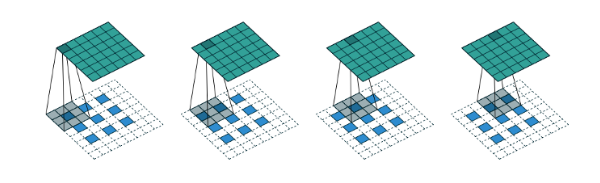
\includegraphics[width=\textwidth,height=0.85\textheight,keepaspectratio]{35.jpg}
			\caption{A convolutional transpose layer example}
		\end{figure}
	\end{frame}
	
	\begin{frame}[plain]
		\begin{figure}
			\centering
			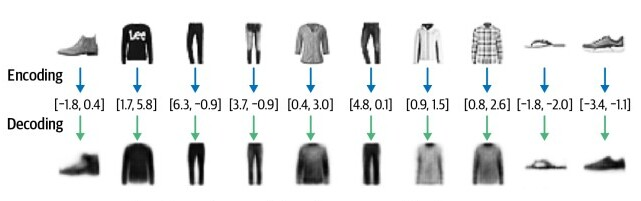
\includegraphics[width=\textwidth,height=0.85\textheight,keepaspectratio]{36.jpg}
			\caption{Examples of encoding and decoding items of clothing}
		\end{figure}
	\end{frame}
	
	\begin{frame}[plain]
		\begin{figure}
			\centering
			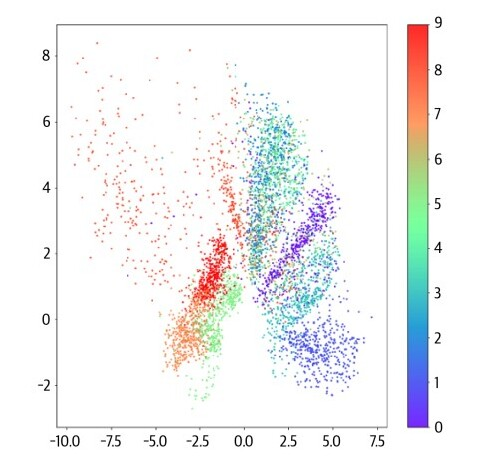
\includegraphics[width=\textwidth,height=0.85\textheight,keepaspectratio]{37.jpg}
			\caption{Plot of the latent space, colored by clothing label}
		\end{figure}
	\end{frame}
	
	\begin{frame}[plain]
		\begin{figure}
			\centering
			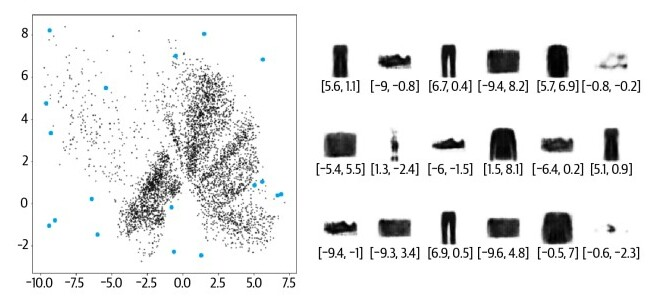
\includegraphics[width=\textwidth,height=0.85\textheight,keepaspectratio]{38.jpg}
			\caption{Generated items of clothing}
		\end{figure}
	\end{frame}
	
	\begin{frame}[plain]
		\begin{figure}
			\centering
			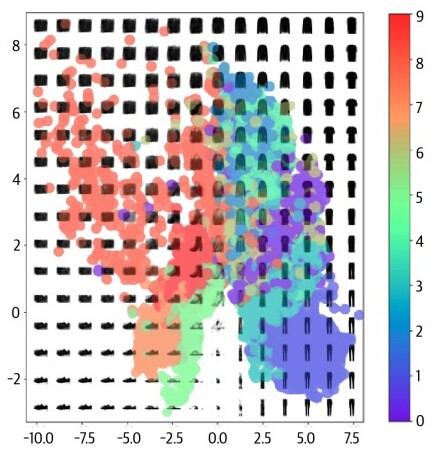
\includegraphics[width=\textwidth,height=0.85\textheight,keepaspectratio]{39.jpg}
			\caption{A grid of decoded embeddings, overlaid with the embeddings from the origi‐
				nal images in the dataset, colored by item type}
		\end{figure}
	\end{frame}
	
	\begin{frame}[plain]
		\begin{figure}
			\centering
			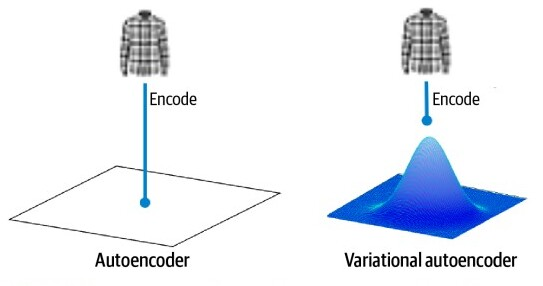
\includegraphics[width=\textwidth,height=0.85\textheight,keepaspectratio]{310.jpg}
			\caption{The difference between the encoders in an autoencoder and a variational
				autoencoder}
		\end{figure}
	\end{frame}
	
	\begin{frame}[plain]
		\begin{figure}
			\centering
			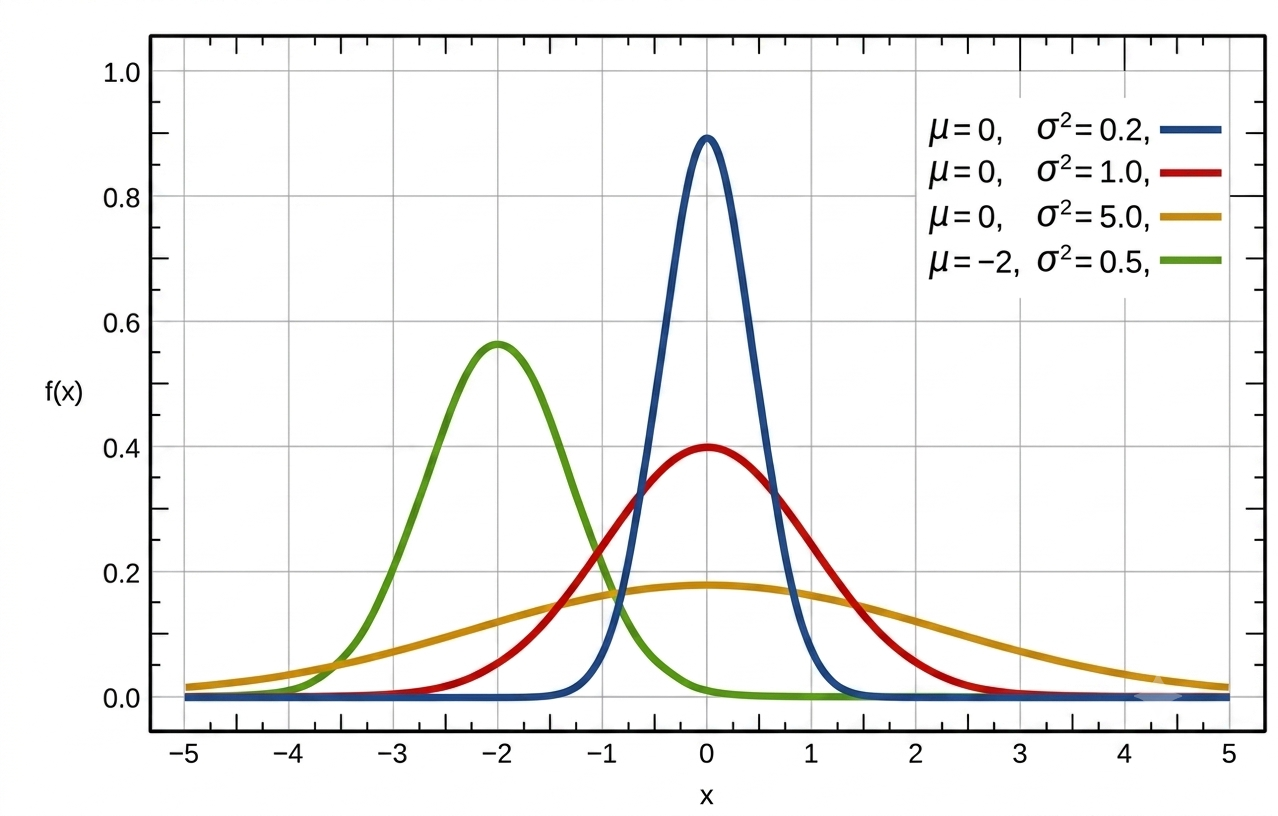
\includegraphics[width=\textwidth,height=0.85\textheight,keepaspectratio]{311.jpg}
			\caption{The normal distribution in one dimension}
		\end{figure}
	\end{frame}
	
	\begin{frame}[plain]
		\begin{figure}
			\centering
			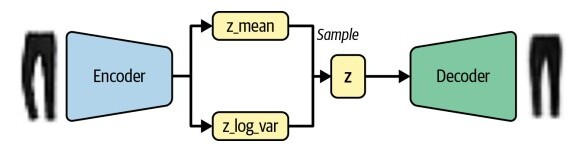
\includegraphics[width=\textwidth,height=0.85\textheight,keepaspectratio]{312.jpg}
			\caption{VAE architecture diagram}
		\end{figure}
	\end{frame}
	
	\begin{frame}[plain]
		\begin{figure}
			\centering
			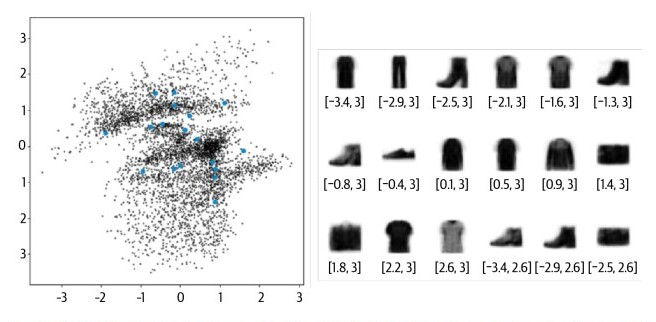
\includegraphics[width=\textwidth,height=0.85\textheight,keepaspectratio]{313.jpg}
			\caption{The new latent space: the black dots show the z\_mean value of each encoded
				image, while blue dots show some sampled points in the latent space (with their decoded
				images on the right)}
		\end{figure}
	\end{frame}
	
	\begin{frame}[plain]
		\begin{figure}
			\centering
			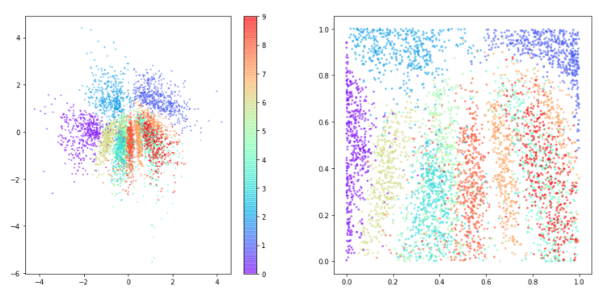
\includegraphics[width=\textwidth,height=0.85\textheight,keepaspectratio]{314.jpg}
			\caption{The latent space of the VAE colored by clothing type}
		\end{figure}
	\end{frame}
	
	\begin{frame}[plain]
		\begin{figure}
			\centering
			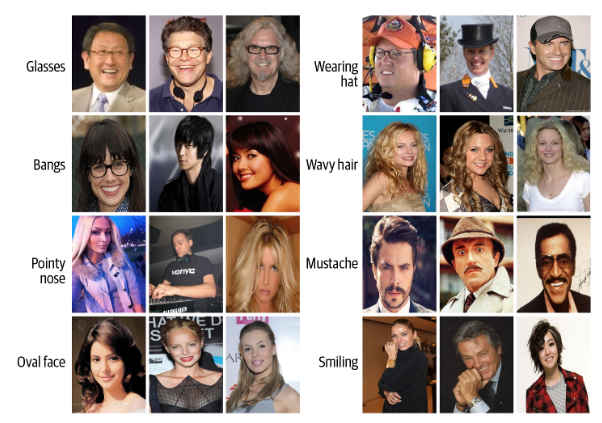
\includegraphics[width=\textwidth,height=0.85\textheight,keepaspectratio]{315.jpg}
			\caption{Some examples from the CelebA dataset}
		\end{figure}
	\end{frame}
	
	\begin{frame}[plain]
		\begin{figure}
			\centering
			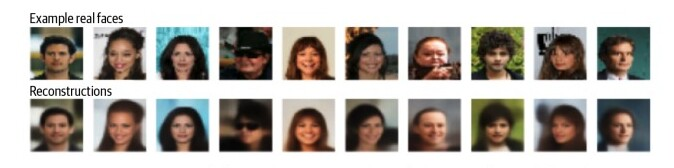
\includegraphics[width=\textwidth,height=0.85\textheight,keepaspectratio]{316.jpg}
			\caption{Reconstructed faces, after passing through the encoder and decoder}
		\end{figure}
	\end{frame}
	
	\begin{frame}[plain]
		\begin{figure}
			\centering
			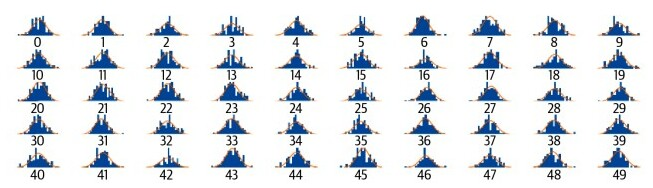
\includegraphics[width=\textwidth,height=0.85\textheight,keepaspectratio]{317.jpg}
			\caption{Distributions of points for the first 50 dimensions in the latent space}
		\end{figure}
	\end{frame}
	
	\begin{frame}[plain]
		\begin{figure}
			\centering
			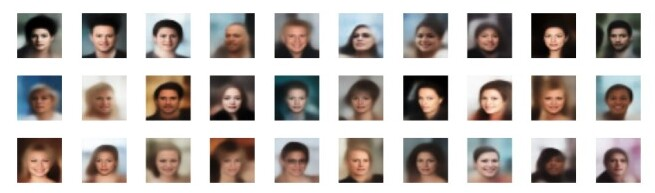
\includegraphics[width=\textwidth,height=0.85\textheight,keepaspectratio]{318.jpg}
			\caption{New generated faces}
		\end{figure}
	\end{frame}
	
	\begin{frame}[plain]
		\begin{figure}
			\centering
			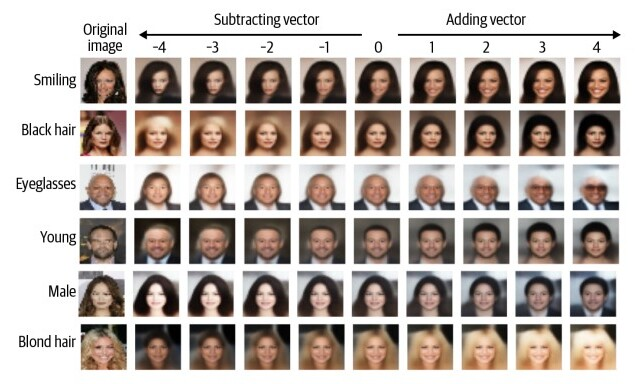
\includegraphics[width=\textwidth,height=0.85\textheight,keepaspectratio]{319.jpg}
			\caption{Adding and subtracting features to and from faces}
		\end{figure}
	\end{frame}
	
	\begin{frame}[plain]
		\begin{figure}
			\centering
			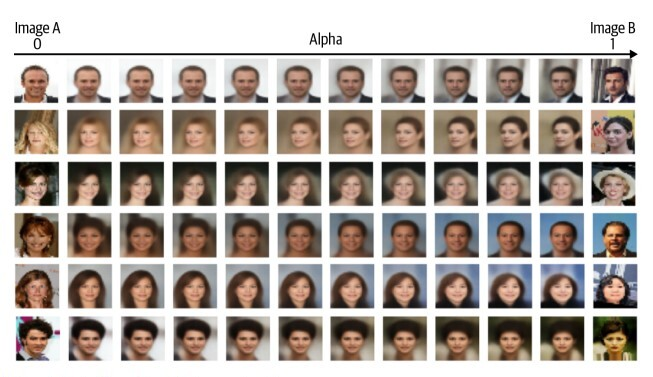
\includegraphics[width=\textwidth,height=0.85\textheight,keepaspectratio]{320.jpg}
			\caption{Morphing between two faces}
		\end{figure}
	\end{frame}
	
\end{document}